\documentclass[11pt,a4paper]{article}
\usepackage[utf8]{inputenc}
\usepackage{amsmath,enumitem,amsfonts,amssymb,graphicx,commath}
\usepackage{sectsty}
\usepackage{multicol}
\usepackage{tikz}
\usetikzlibrary{shapes,arrows,automata,arrows.meta}

\graphicspath{ {./img/} }
\DeclareMathAlphabet{\pazocal}{OMS}{zplm}{m}{n}

\usepackage[%
    left=1in,%
    right=1.0in,%
    top=0.8in,%
    bottom=1in,%
]{geometry}%

\sectionfont
{\fontsize{14.4}{12}\selectfont}
\title{\textbf{Principles of AI Planning
		\\{\Large Exercise Sheet 11}}}
\makeatletter
\renewcommand{\@maketitle}
{
	\newpage
	\null
	\vskip 2em%
	\begin{center}%
		{\LARGE \@title \\ \par}%
	\end{center}%
	\par
} \makeatother

\begin{document}
\begin{flushleft}
	Authors:\\
	Erick Rosete Beas | er165@uni-freiburg.de\\
	Jessica Lizeth Borja Diaz | jb986@uni-freiburg.de\\
\end{flushleft}
{\let\newpage\relax\maketitle}
\begin{center} 
	\large 24.01.2020
\end{center}


%%%%%%%%%%%%%%%%%%%%%  Ejercicio 1 %%%%%%%%%%%%%%%%%%%%%%%%%
\section*{Exercise 11.1 - Strong stubborn sets}
Consider the $SAS^+$ planning task $\Pi$ with variables 
$V =\{pos,left,right,hat \}, \pazocal{D}_{pos}=\{
home,uni\}$ and $\pazocal{D}_{left}=\pazocal{D}_{right}=\pazocal{D}_{hat}
=\{t,f\}$. The initial state $I = \{pos \mapsto home, left \mapsto f,
right \mapsto f, hat \mapsto f\}$ and the goal specification is
$\gamma = \{pos \mapsto uni\}$. There are four operators in O, namely

\[ \begin{array}{rcl}
	\mbox{wear-left-shoe (WLS)}  & = & \langle pos=home \land left = f, left:=t \rangle\\
	\mbox{wear-right-shoe (WRS)} & = & \langle pos=home \land right = f, right:=t \rangle\\
	\mbox{wear-hat (WH)} 	   & = & \langle pos=home \land hat = f, hat:=t \rangle\\
	\mbox{go-to-university (GU)}& = & \langle pos=home \land left = t \land right = t, pos:=uni \rangle\\
\end{array}\] 

(a) Draw the breadth-first search graph (with duplicate detection) for planning
task $\Pi$ without any form of partial-order reduction.
\begin{center}
	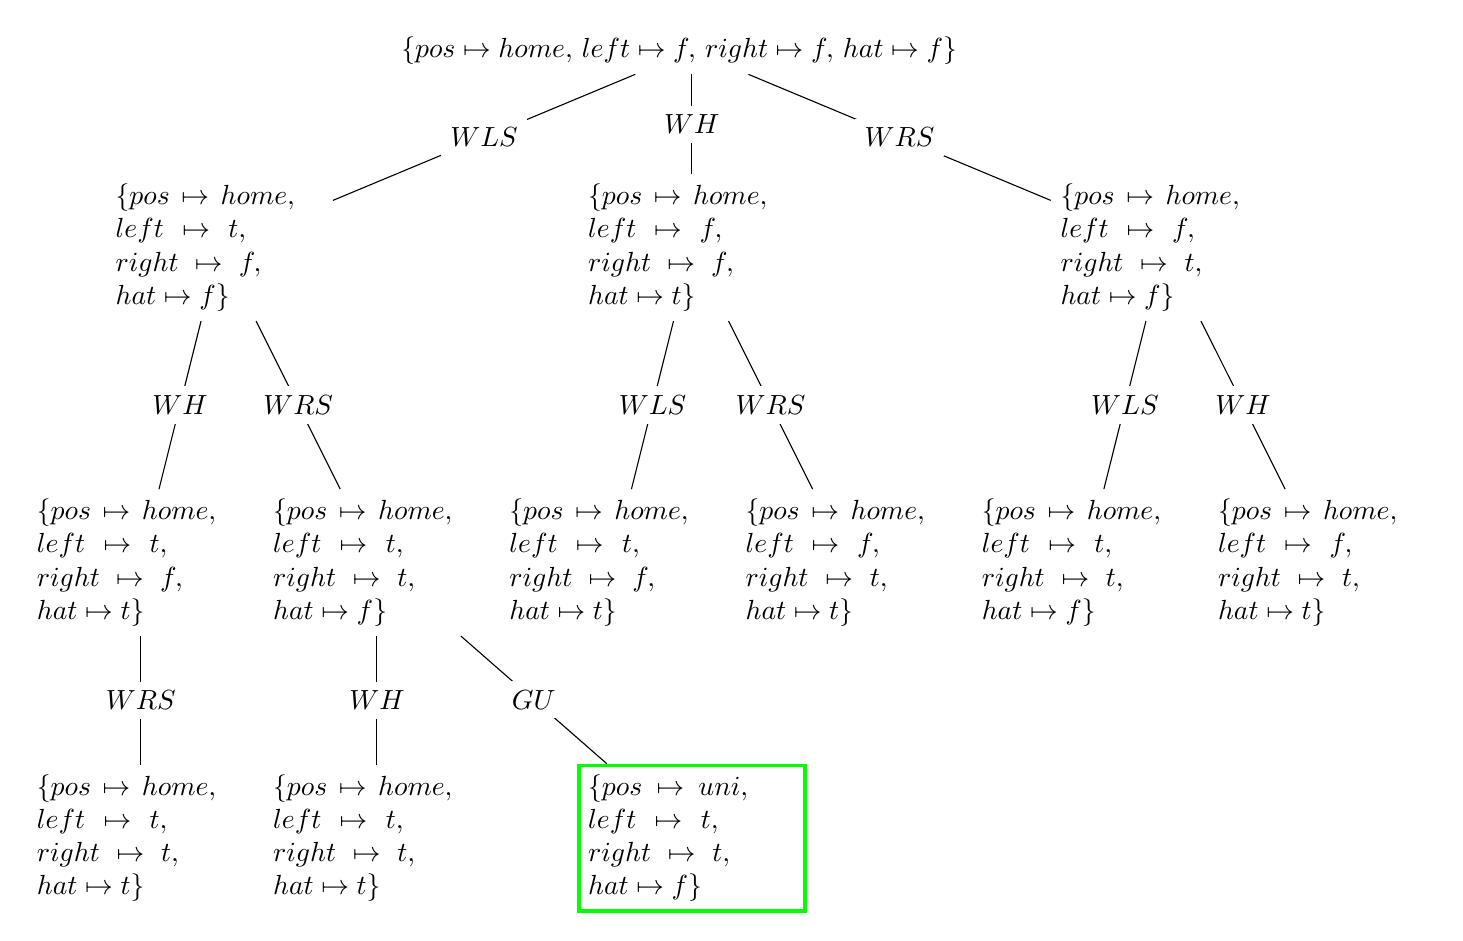
\begin{tikzpicture}
		\begin{scope}
            [
                every node/.style={
					text width = 7.5em },
				active/.style = {draw=green,text= black, very thick}
            ]
            
			\node(a)[text width = 21em] at (0,0) {$\{pos \mapsto home,$ $left\mapsto f,$ $right \mapsto f ,$ $hat \mapsto f \}$};
			
			\node(b) at (-6,-2.5) {$\{pos \mapsto home,$  $left\mapsto t,$  $right \mapsto f ,$ $hat \mapsto f \}$};
            \node(c) at (0,-2.5) {$\{pos \mapsto home,$ $left\mapsto f,$ $right \mapsto f ,$ $hat \mapsto t \}$};
			\node(d) at (6,-2.5) {$\{pos \mapsto home,$ $left\mapsto f,$ $right \mapsto t ,$ $hat \mapsto f \}$};
			
			\node(e) at (-7,-6.5) {$\{pos \mapsto home,$ $left\mapsto t,$ $right \mapsto f ,$ $hat \mapsto t \}$};
			\node(f) at (-4,-6.5) {$\{pos \mapsto home,$ $left\mapsto t,$ $right \mapsto t ,$ $hat \mapsto f \}$};
			\node(g) at (-1,-6.5) {$\{pos \mapsto home,$ $left\mapsto t,$ $right \mapsto f ,$ $hat \mapsto t \}$};
			\node(h) at (2,-6.5) {$\{pos \mapsto home,$ $left\mapsto f,$ $right \mapsto t ,$ $hat \mapsto t \}$};
			\node(i) at (5,-6.5) {$\{pos \mapsto home,$ $left\mapsto t,$ $right \mapsto t ,$ $hat \mapsto f \}$};
			\node(j) at (8,-6.5) {$\{pos \mapsto home,$ $left\mapsto f,$ $right \mapsto t ,$ $hat \mapsto t \}$};

			\node(k) at (-7,-10) {$\{pos \mapsto home,$ $left\mapsto t,$ $right \mapsto t ,$ $hat \mapsto t \}$};
			\node(l) at (-4,-10) {$\{pos \mapsto home,$ $left\mapsto t,$ $right \mapsto t ,$ $hat \mapsto t \}$};
			\node(m)[active] at (0,-10) {$\{pos \mapsto uni,$ $left\mapsto t,$ $right \mapsto t ,$ $hat \mapsto f \}$};

		\end{scope}
		\begin{scope}
            [>={Stealth[black]},
                every node/.style={fill=white},
                every edge/.style={draw=black,text=black},
				active/.style = {draw=green,text= black, very thick}
            ]
            \path 
            (a) edge         node{$WLS$}(b)
            (a) edge         node{$WH$}(c)
			(a) edge         node{$WRS$}(d)
			(b) edge         node{$WH$}(e)
			(b) edge         node{$WRS$}(f)
			(c) edge         node{$WLS$}(g)
			(c) edge         node{$WRS$}(h)
			(d) edge         node{$WLS$}(i)
			(d) edge         node{$WH$}(j)
			(e) edge         node{$WRS$}(k)
			(f) edge         node{$WH$}(l)
			(f) edge         node{$GU$}(m);
		\end{scope}
    \end{tikzpicture}
\end{center}

(b) Draw the breadth-first search graph (with duplicate detection) for planning task $\Pi$ using
strong stubborn set pruning. For each expansion of a node for a state $s$, specify in detail how
$T_s$ (and thus $T_{app(s)}$) are computed, i.e., explain how the initial disjunctive action landmark
is chosen and how operators are iteratively added to $T_s$ as part of necessary enabling sets or
interfering operators, respectively. Break ties in favor of \emph{wear-left-shoe} over \emph{wear-right-shoe.}\\

\textbf{How many node expansion do you save with strong stubborn sets compared to plain breadthfirst search?
 What about the lengths of the resulting solutions?}\\

\begin{center}
	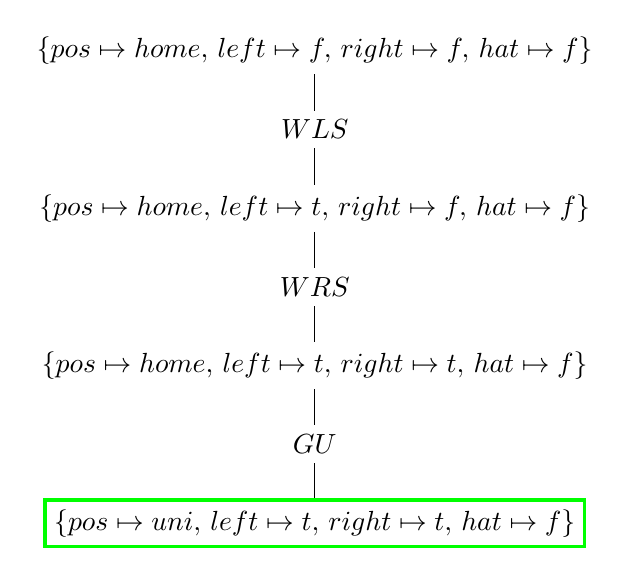
\begin{tikzpicture}
		\begin{scope}
            [
                every node/.style={minimum width = 7.5em },
				active/.style = {draw=green,text= black, very thick}
            ]
            
			\node(a) at (0,0) {$\{pos \mapsto home,$ $left\mapsto f,$ $right \mapsto f ,$ $hat \mapsto f \}$};
			
			\node(b) at (0,-2) {$\{pos \mapsto home,$  $left\mapsto t,$  $right \mapsto f ,$ $hat \mapsto f \}$};
			\node(f) at (0,-4) {$\{pos \mapsto home,$ $left\mapsto t,$ $right \mapsto t ,$ $hat \mapsto f \}$};
			\node(m)[active] at (0,-6) {$\{pos \mapsto uni,$ $left\mapsto t,$ $right \mapsto t ,$ $hat \mapsto f \}$};

		\end{scope}
		\begin{scope}
            [>={Stealth[black]},
                every node/.style={fill=white},
                every edge/.style={draw=black,text=black},
            ]
            \path 
            (a) edge         node{$WLS$}(b)
			(b) edge         node{$WRS$}(f)
			(f) edge         node{$GU$}(m);
		\end{scope}
    \end{tikzpicture}
\end{center}

%%%%%%%%%%%%%%%%%%%%%  Ejercicio 2 %%%%%%%%%%%%%%%%%%%%%%%%%
\section*{Exercise 11.2 - Weak vs. strong stubborn sets}
Show that \emph{weak} stubborn sets admint exponentially more pruning than
\emph{strong} stubborn sets.\\


\end{document}